\documentclass[12pt,addpoints]{evalua}
\grado{1$^\circ$ de Secundaria}
\cicloescolar{2023-2024}
\materia{Matemáticas 1}
\unidad{1}
\title{Examen de la Unidad}
\aprendizajes{
        \item Convierte fracciones decimales a notación decimal y viceversa. Aproxima algunas fracciones no decimales usando la notación decimal. 
        \item Ordena fracciones y números decimales.
     \item Resuelve problemas de suma y resta con números enteros, fracciones y decimales positivos y negativos.
\item Resuelve problemas de multiplicación con fracciones y decimales y de división con decimales.
}
     \author{Prof.: Julio César Melchor Pinto}
\begin{document}
\begin{questions}
      \question[10] Escribe sobre la línea el símbolo de mayor que ($>$), menor que ($<$), o igual ($=$) según corresponda.
      \begin{multicols}{2}
            \begin{parts}
                  \part $\dfrac{2}{5}$ \fillin[$>$][0.5in] $\dfrac{1}{3}$\\[0.75em]
                  \part $\dfrac{3}{4}$ \fillin[$<$][0.5in] $\dfrac{4}{5}$\\[0.75em]
                  \part $\dfrac{2}{5}$ \fillin[$<$][0.5in] $\dfrac{2}{3}$\\[0.75em]
                  \part $\dfrac{3}{2}$ \fillin[$=$][0.5in] $\dfrac{9}{6}$\\[0.75em]
                  \part $\dfrac{5}{6}$ \fillin[$>$][0.5in] $\dfrac{4}{6}$\\[0.75em]
                  % \part $\dfrac{4}{3}$ \fillin[$>$][0.5in] $\dfrac{5}{4}$\\[0.75em]
                  % \part $\dfrac{1}{3}$ \fillin[$=$][0.5in] $\dfrac{9}{3}$\\[0.75em]
                  % \part $\dfrac{2}{3}$ \fillin[$<$][0.5in] $\dfrac{3}{2}$\\[0.75em]
                  % \part $\dfrac{3}{4}$ \fillin[$>$][0.5in] $\dfrac{2}{3}$\\[0.75em]
                  % \part $\dfrac{5}{6}$ \fillin[$>$][0.5in] $\dfrac{4}{5}$\\[0.75em]
                  \part $-51$ \fillin[$>$][0.5in] $-55$\\[0.75em]
                  \part $-77$ \fillin[$>$][0.5in] $-177$\\[0.75em]
                  \part $-100$ \fillin[$<$][0.5in] $-99$\\[0.75em]
                  \part $-182$ \fillin[$>$][0.5in] $-189$\\[0.75em]
                  \part $-97$ \fillin[$<$][0.5in] $-96.2$\\[0.75em]
                  % \part $-36$ \fillin[$>$][0.5in] $-39$\\[0.75em]
                  % \part $-3.5$ \fillin[$<$][0.5in] $-2.2$\\[0.75em]
                  % \part $-12$ \fillin[$<$][0.5in] $-11$\\[0.75em]
                  % \part $-10.001$ \fillin[$>$][0.5in] $-100.01$\\[0.75em]
                  % \part $-0.99$ \fillin[$>$][0.5in] $1.01$\\[0.75em]
            \end{parts}
      \end{multicols}

      \newpage
      \question[10] Calcula lo que se te pide en cada inciso.
      \begin{multicols}{2}
            \begin{parts}
                  % \part Encuentra el mínimo común múltiplo de 2 y 9.   \\[1em]
                  % \part Encuentra el máximo común divisor de 5 y 15.   \\[1em]
                  % \part Encuentra el mínimo común múltiplo de 2 y 5.    \\[1em]
                  % \part Encuentra el máximo común divisor de 33 y 121.  \\[1em]
                  % \part Encuentra el máximo común divisor de 25 y 100.  \\[1em]
                  \part Encuentra el máximo común divisor de 18 y 36.
                  \begin{solutionbox}{2.5cm}
                        El máximo común divisor de 18 y 36 es 18.
                  \end{solutionbox}
                  \part Encuentra el mínimo común múltiplo de 6 y 7.
                  % \part Encuentra el mínimo común múltiplo de 4 y 9.    \\[1em]
                  \begin{solutionbox}{2.5cm}
                        El mínimo común múltiplo de 6 y 7 es 42.
                  \end{solutionbox}
                  \part Encuentra el mínimo común múltiplo de 2, 3 y 4.
                  \begin{solutionbox}{2.5cm}
                        El mínimo común múltiplo de 2, 3 y 4 es 12.
                  \end{solutionbox}
                  \part Encuentra el máximo común divisor de 2 y 14.
                  \begin{solutionbox}{2.5cm}
                        El máximo común divisor de 2 y 14 es 2.
                  \end{solutionbox}
            \end{parts}
      \end{multicols}

      \question[10] Escribe el número que representa el punto indicado en la recta numérica de cada uno de los siguientes incisos.

      \begin{multicols}{2}
            \begin{parts}
                  \part 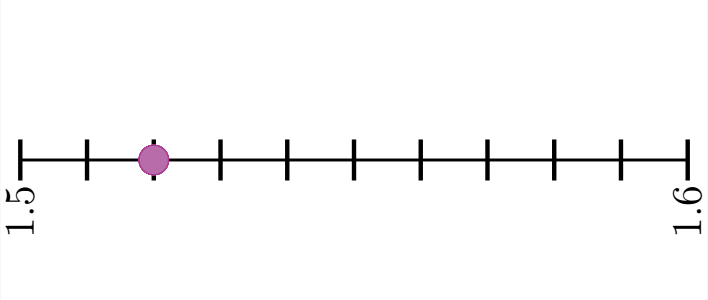
\includegraphics[width=150px]{../images/recta_num_1.52.png} \\[-0.5em] \fillin[$1.52$][1.5in]   \\[-1.4em]
                  \part 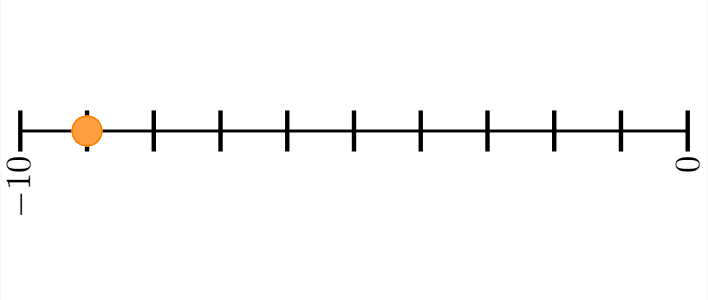
\includegraphics[width=150px]{../images/recta_num_-9.png}   \\[-0.5em] \fillin[$-9$][1.5in]     \\[-1.4em]
                  \part 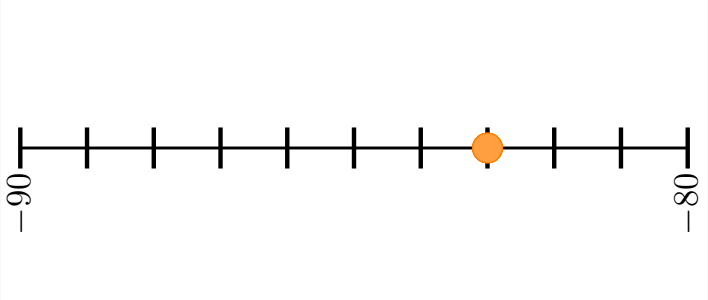
\includegraphics[width=150px]{../images/recta_num_-83.png}  \\[-0.5em]  \fillin[$-83$][1.5in]   \\[-1.4em]
                  \part 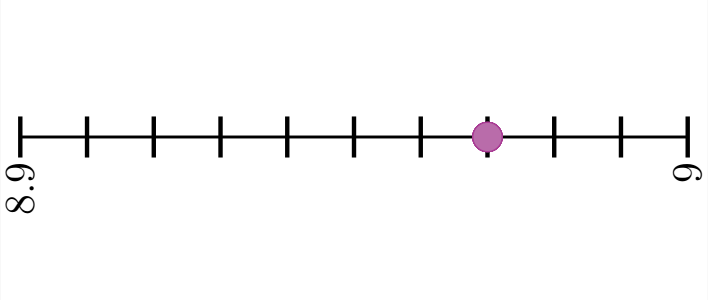
\includegraphics[width=150px]{../images/recta_num_8.97.png} \\[-0.5em]  \fillin[$8.97$][1.5in]  \\[-1.4em]
                  \part 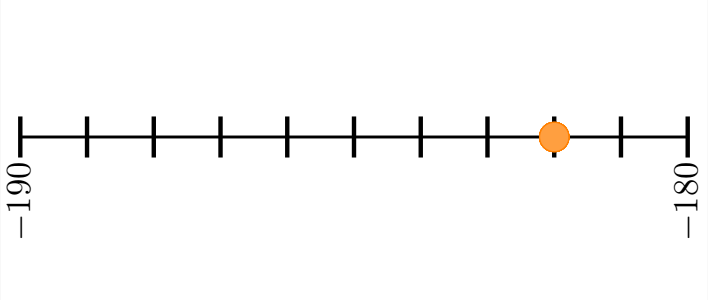
\includegraphics[width=150px]{../images/recta_num_-182.png} \\[-0.5em]   \fillin[$-182$][1.5in] \\[-1.4em]
                  \part 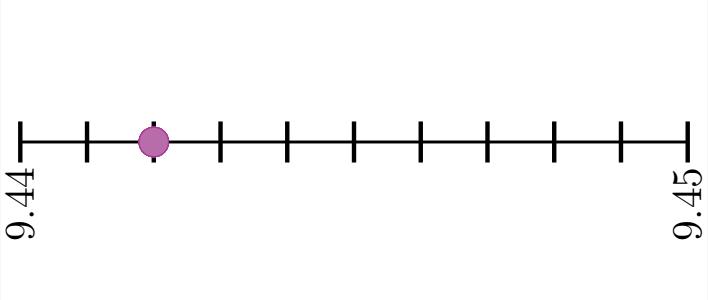
\includegraphics[width=150px]{../images/recta_num_9.442.png}\\[-0.5em]  \fillin[$9.44$][1.5in]  \\[-1.4em]
                  \part 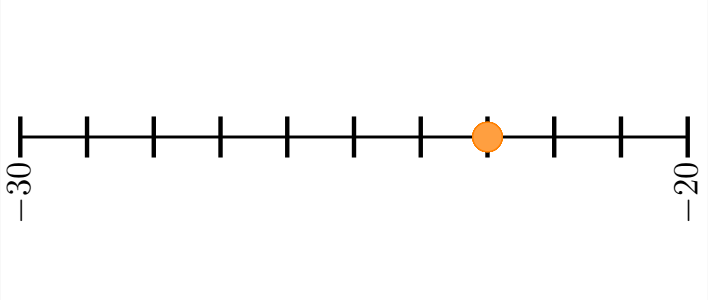
\includegraphics[width=150px]{../images/recta_num_-23.png}  \\[-0.5em]  \fillin[$-23$][1.5in]   \\[-1.4em]
                  \part 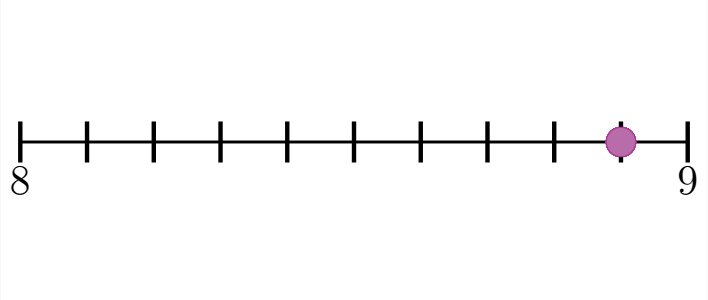
\includegraphics[width=150px]{../images/recta_num_8.9.png}  \\[-0.5em]  \fillin[$8.9$][1.5in]   \\[-1.4em]
                  \part 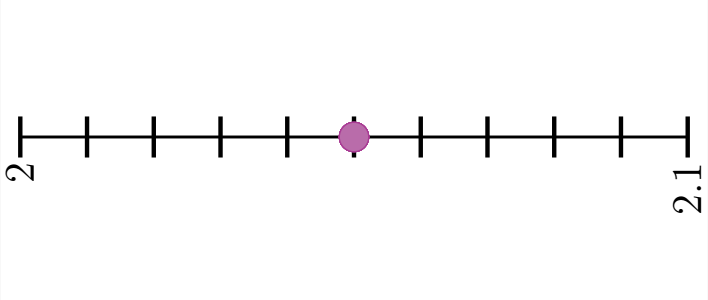
\includegraphics[width=150px]{../images/recta_num_2.05.png} \\[-0.5em]  \fillin[$2.05$][1.5in]  \\[-1.4em]
                  \part 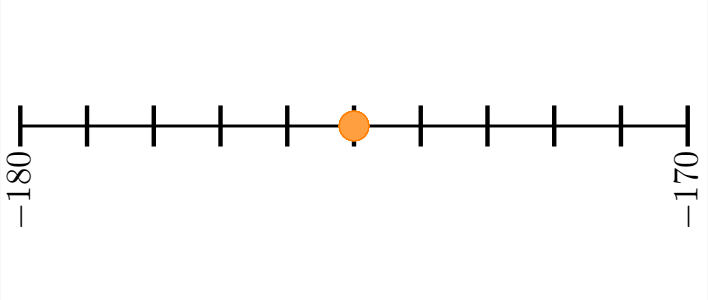
\includegraphics[width=150px]{../images/recta_num_-175.png} \\[-0.5em]   \fillin[$-175$][1.5in]
                  % \part 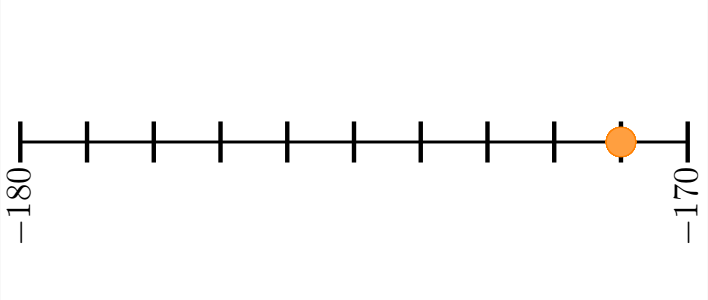
\includegraphics[width=130px]{../images/recta_num_-171.png}   \fillin[$-171$][1.5in]
                  % \part 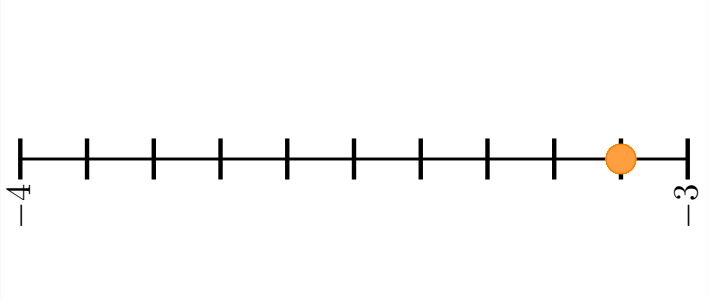
\includegraphics[width=130px]{../images/recta_num_-3.1.png}   \fillin[$-3.1$][1.5in]
                  % \part 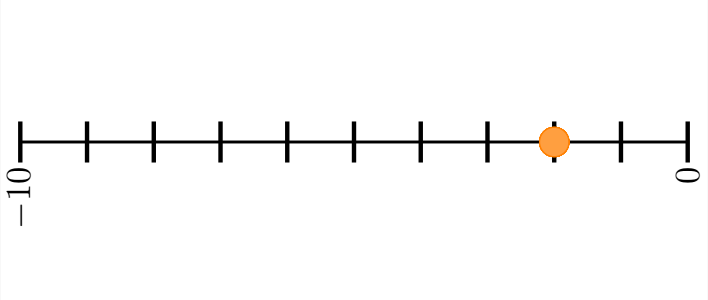
\includegraphics[width=130px]{../images/recta_num_-2.png}   \fillin[$-2$][1.5in]
                  % \part 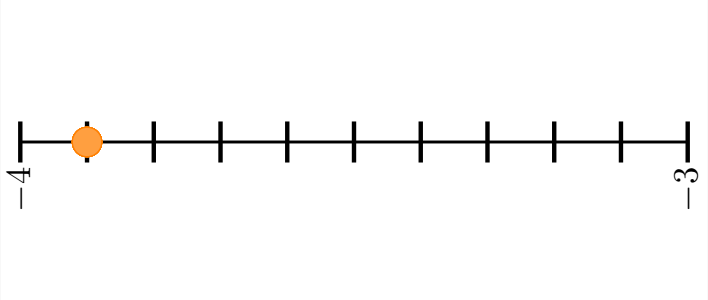
\includegraphics[width=130px]{../images/recta_num_-3.9.png}   \fillin[$-3.9$][1.5in]
                  % \part 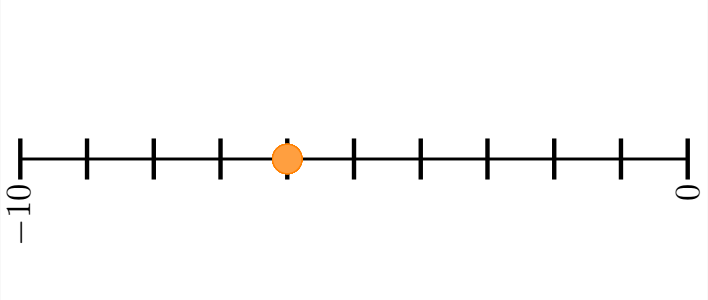
\includegraphics[width=130px]{../images/recta_num_-6.png}   \fillin[$-6$][1.5in]
                  % \part 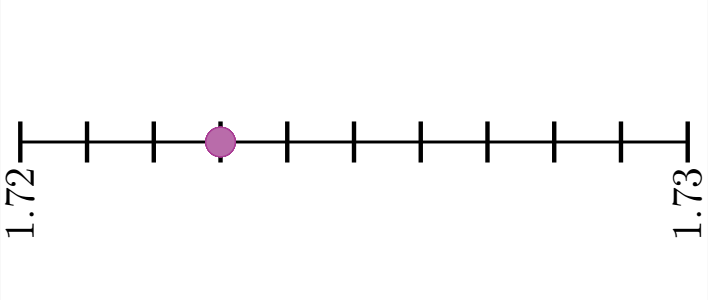
\includegraphics[width=130px]{../images/recta_num_1.723.png} \fillin[$1.723$][1.5in]
                  % \part 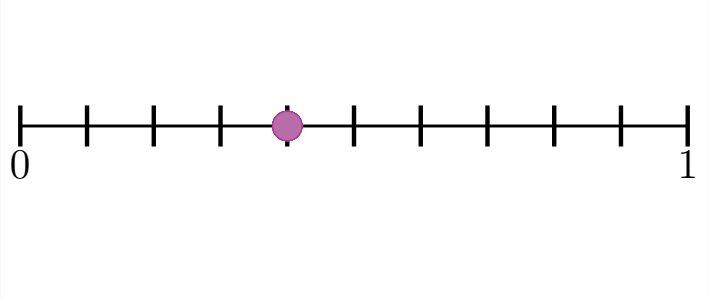
\includegraphics[width=130px]{../images/recta_num_0.4.png}   \fillin[$0.4.$][1.5in]
                  % \part 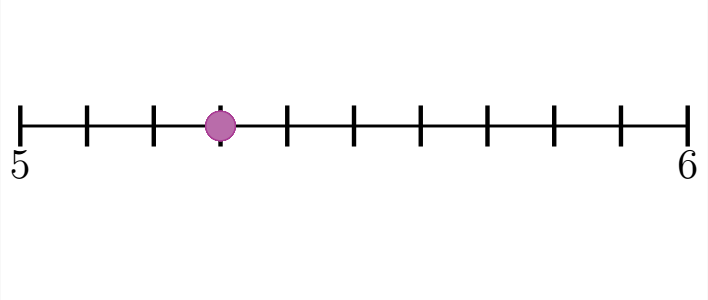
\includegraphics[width=130px]{../images/recta_num_5.3.png}   \fillin[$5.3.$][1.5in]
                  % \part 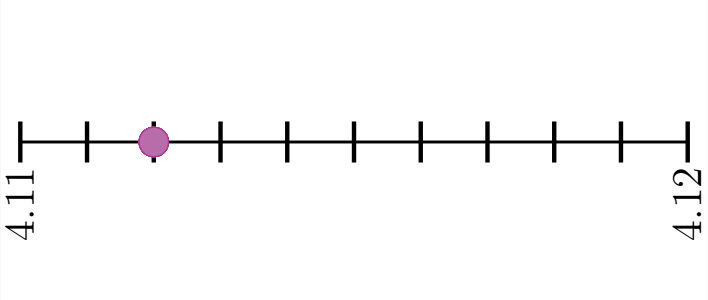
\includegraphics[width=130px]{../images/recta_num_4.112.png} \fillin[$4.11$][1.5in]
                  % \part 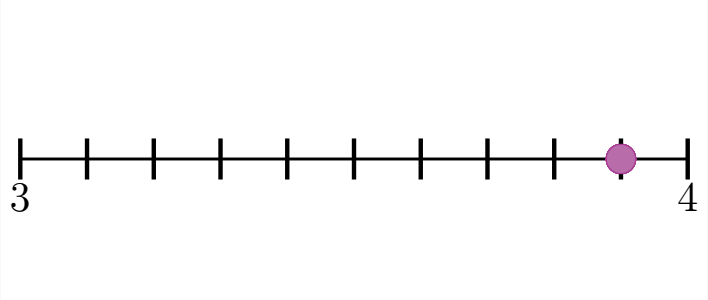
\includegraphics[width=130px]{../images/recta_num_3.9.png}   \fillin[$3.9.$][1.5in]
            \end{parts}
      \end{multicols}

      \question[15] Escribe el número decimal que representa a la fracción y viceversa en cada uno de los siguientes incisos.
      \begin{multicols}{2}
            \begin{parts}
                  % \part $\dfrac{5}{4}=$         \fillin[$1.25$][1in]          \\[1em]
                  % \part $\dfrac{7}{20}=$        \fillin[$0.35$][1in]         \\[1em]
                  % \part $\dfrac{1927}{1000}=$   \fillin[$1.927$][1in]   \\[1em]
                  % \part $\dfrac{9}{4}=$         \fillin[$2.25$][1in]          \\[1em]
                  % \part $\dfrac{3}{20}=$        \fillin[$0.15$][1in]         \\[1em]
                  \part $\dfrac{13}{100}=$      \fillin[$0.13$][1in]       \\[1em]
                  \part $\dfrac{11}{50}=$       \fillin[$0.22$][1in]        \\[1em]
                  \part $\dfrac{459}{100}=$    \fillin[$4.59$][1in]    \\[1em]
                  \part $\dfrac{19}{25}=$       \fillin[$0.76$][1in]        \\[1em]
                  \part $\dfrac{2039}{1000}=$   \fillin[$2.039$][1in]   \\[1em]
                  \part $0.04=$      \fillin[$\dfrac{1}{25}$][1in]       \\[1em]
                  \part $0.875=$       \fillin[$\dfrac{7}{8}$][1in]        \\[1em]
                  \part $0.45=$    \fillin[$\dfrac{9}{20}$][1in]    \\[1em]
                  \part $0.002=$      \fillin[$\dfrac{1}{500}$][1in]       \\[1em]
                  \part $0.9=$       \fillin[$\dfrac{9}{10}$][1in]        \\[1em]
            \end{parts}
      \end{multicols}

      \question[20] Realiza la siguiente operación con números negativos.
      \begin{multicols}{2}
            \begin{parts}
                  \part $-90+25=$  \fillin[$-65$][0.5in]  \\[1em]
                  % \part $-16-99=$  \fillin[$-115$][0.5in] \\[1em]
                  % \part $-137-350=$ \fillin[$-487$][0.5in] \\[1em]
                  % \part $203-661=$    \fillin[$-458$][0.5in]  \\[1em]
                  \part $-223+67=$ \fillin[$-156$][0.5in]   \\[1em]
                  % \part $-68+29=$ \fillin[$-39$][0.5in]    \\[1em]
                  % \part $-416-90=$ \fillin[$-506$][0.5in]    \\[1em]
                  % \part $-64-94=$ \fillin[$-158$][0.5in]    \\[1em]
                  \part $-91-209=$ \fillin[$-300$][0.5in]    \\[1em]
                  \part $12-107=$ \fillin[$-95$][0.5in]    \\[1em]
                  \part $(64)-(-231)+(87)=$ \fillin[$382$][0.5in]  \\[1em]
                  \part $(-16)+(-81)=$ \fillin[$-97$][0.5in] \\[1em]
                  \part $(121)-(54)+(-14)=$ \fillin[$53$][0.5in]  \\[1em]
                  % \part $(49)-(314)+(-191)=$ \fillin[$-456$][0.5in]  \\[1em]
                  % \part $(-13)-(91)=$ \fillin[$-104$][0.5in]  \\[1em]
                  \part $(-97)+(55)=$ \fillin[$-42$][0.5in]  \\[1em]
                  % \part $(54)+(-97)+(-71)=$ \fillin[$-114$][0.5in]  \\[1em]
                  \part $(57)+(-211)-(-81)=$ \fillin[$-73$][0.5in]  \\[1em]
                  \part $(134)-(-94)=$ \fillin[$228$][0.5in]  \\[1em]
                  % \part $7457-841-3872$ \fillin[$2744$][0.5in] \\[1em]
            \end{parts}
      \end{multicols}

      \question[15] Realiza las siguientes operaciones.
      \begin{multicols}{2}
            \begin{parts}
                  \part $2381 \divisionsymbol 1000=$ \fillin[$2.381$][0.5in] \\[1em]
                  % \part $32 \times 100=$ \fillin[$3200$][0.5in] \\[1em]
                  % \part $3461 \divisionsymbol 1000=$ \fillin[$3.461$][0.5in] \\[1em]
                  \part $0.09 \times 100=$ \fillin[$9$][0.5in] \\[1em]
                  \part $\dfrac{3}{10}+\dfrac{4}{5}=$ \fillin[$\dfrac{11}{10}$ o 1$\dfrac{1}{10}$][0.5in] \\[1em]
                  % \part $\dfrac{3}{4}-\dfrac{2}{5}=$ \fillin[$\dfrac{7}{20}$][0.5in] \\[1em]
                  \part $\dfrac{2}{3}-\dfrac{2}{5}=$ \fillin[$\dfrac{4}{15}$][0.5in] \\[1em]
                  % \part $\dfrac{3}{8}+\dfrac{7}{10}=$ \fillin[$\dfrac{43}{40}$ o 1$\dfrac{3}{40}$][0.5in] \\[1em]
                  % \part $\dfrac{7}{10}+\dfrac{2}{5}=$ \fillin[$\dfrac{11}{10}$ o 1$\dfrac{1}{10}$][0.5in] \\[1em]
                  % \part $\dfrac{3}{4}-\dfrac{2}{5}=$ \fillin[$\dfrac{7}{20}$][0.5in] \\[1em]  
                  \part $3\dfrac{1}{2}-1\dfrac{1}{3}$ \fillin[$2\dfrac{1}{6}$][0.5in] \\[1em]
                  % \part $2\frac{2}{3}-2\frac{2}{5}$ \fillin[$\dfrac{4}{15}$][0.5in] \\[1em]
            \end{parts}
      \end{multicols}

      \newpage

      \question[20] Contesta la pregunta en cada uno de los siguientes problemas.
      \begin{multicols}{2}
            \begin{parts}
                  \part María y Jorge tienen 45 bolas blancas, 15 bolas azules y 90 bolas rojas y quieren hacer el mayor número de collares iguales sin que sobre ninguna bola. \textbf{¿Cuántos collares iguales pueden hacer?}
                  \begin{solutionbox}{4.5cm}
                        El numero de collares iguales que pueden hacer se calcula con el máximo común divisor de 45, 15 y 90, ya que es la cantidad más grande en que se puede dividir cada uno de los números sin que sobre ninguna bola.
                        \begin{align*}
                              \text{MCD}(45,15,90) & = 15
                        \end{align*}
                        Por lo tanto, pueden hacer 15 collares iguales.
                  \end{solutionbox}

                  \part Andrés tiene una cuerda de 256 metros y otra de 192 metros. Desea cortarlas de modo que todos los trozos sean iguales pero lo más largos posible. \textbf{¿Cuántos trozos de la cuerda de 256 metros obtendrá?}
                  \begin{solutionbox}{5.5cm}
                        El tamaño de los trozos que obtendrá se calcula con el máximo común divisor de 256 y 192, ya que es la cantidad más grande en que se puede dividir cada uno de los números sin que sobre ninguna cuerda.
                        \begin{align*}
                              \text{MCD}(256,192) & = 64
                        \end{align*}
                        Entonces, si dividimos la cuerda de 256 metros en trozos de 64 metros, obtendrá 4 trozos.
                  \end{solutionbox}

                  % \part Un carpintero quiere cortar una plancha de madera de 252 cm de largo y 180 cm de ancho, en cuadrados lo más grandes posible. \textbf{¿Cuál debe ser la longitud del lado de cada cuadrado?}
                  % \part Alan y Pedro comen en el mismo restaurante, pero Alan asiste cada 20 días y Pedro cada 30. \textbf{¿Cuándo volverán a encontrarse?}
                  \part Un automóvil viaja a 112.4 kilómetros por hora en una carretera. \textbf{¿Qué distancia recorre en 4 horas?}
                  \begin{solutionbox}{3.5cm}
                        Si el automóvil recorre 112.4 kilómetros cada hora, en 4 horas recorrerá:
                        \begin{align*}
                              112.4 \times 4 & = 449.6
                        \end{align*}
                        Por lo tanto, recorrerá 449.6 kilómetros.
                  \end{solutionbox}



                  % \part Si el millar de hojas de papel tiene un costo de 813 pesos, \textbf{¿cuál es el precio por una sola hoja?}

                  \part Los gastos del Arturo, en cierto mes, fueron los siguientes: 1,200 pesos de renta, 925.62 pesos de comida, 120.85 pesos de lavandería, 104.73 pesos en transporte y 259.51 pesos de ahorros. \textbf{¿Cuánto gastó Arturo en ese mes?}
                  \begin{solutionbox}{3.5cm}
                        Para conocer el gasto total de Arturo, se suman todos los gastos que tuvo en ese mes.
                        \begin{align*}
                              1,200 + 925.62 + 120.85 + 104.73 + 259.51 & = 2,610.71
                        \end{align*}
                        Por lo tanto, gastó 2,610.71 pesos.
                  \end{solutionbox}

                  %\part Luis pagó 94.50 pesos en una sala de videojuegos, en donde por esa cantidad le dieron 21 fichas para jugar. \textbf{¿Cuál es el precio que pagó por una ficha?}
                  %\part La mamá de Susana compró 11 metros de franela y pagó 103.40 pesos. \textbf{¿Cuánto cuesta el metro de franela?}
                  % \part El precio de 385 artículos comerciales es de 1,232 pesos. \textbf{¿Cuál es el precio unitario de cada artículo?}
                  \part Ricardo ha pagado por una agenda, pluma y una libreta 248.6 pesos. Si la agenda le costó 120.2 pesos, la pluma le costó 18.3 pesos, \textbf{¿cuánto costó la libreta?}
                  \begin{solutionbox}{4cm}
                        El precio de la libreta se calcula restando el precio de la agenda y la pluma al total que pagó Ricardo.
                        \begin{align*}
                              248.6 - 120.2 - 18.3 & = 110.1
                        \end{align*}
                        Por lo tanto, la libreta costó 110.1 pesos.
                  \end{solutionbox}

                  % \part Una computadora tiene un disco duro de 368 GB de memoria, si varios programas ocupan 128.75 GB. \textbf{¿Qué cantidad de memoria está libre?}
                  % \part Una pintura tiene un costo de 25.75 pesos el litro, una persona compra 48 litros. \textbf{¿Cuánto debe pagar?}

                  \part Los alumnos de secundaria van a comprar un balón de fútbol que cuesta 437.50 pesos. Si son un total de 35 alumnos, \textbf{¿con cuánto dinero debe cooperar cada alumno?}
                  \begin{solutionbox}{4.5cm}
                        El dinero que debe cooperar cada alumno se calcula dividiendo el precio del balón entre el número de alumnos.
                        \begin{align*}
                              \dfrac{437.50}{35} & = 12.5
                        \end{align*}
                        Por lo tanto, cada alumno debe cooperar con 12.5 pesos.
                  \end{solutionbox}
            \end{parts}
      \end{multicols}
\end{questions}
\end{document}